\section{Construction de nouvelles lois}

En combinant des lois normales, on peut créer de nouvelles lois de probabilités utiles en statistique :

\subsection{Somme de lois normales}

\begin{proposition}{}{}
	Soient deux variables aléatoires indépendantes $X_1 \sim \mathcal{N}(\mu_1,\sigma_1)$ et $X_2 \sim \mathcal{N}(\mu_2,\sigma_2)$, $a>0$ :
	\begin{enumerate}
		\item $X_1+X_2$ suit une loi $\mathcal{N}(\mu_1+\mu_2,\sqrt{\sigma_1^2+\sigma_2^2})$
		\item $aX_1$ suit une loi $\mathcal{N}(a\mu_1,|a|\sigma_1)$
		\item $-X_1$ suit une loi $\mathcal{N}(-\mu_1,+\sigma_1)$
		
	\end{enumerate}
	
\end{proposition}

\begin{exemple}{}{}
	Si $X_1$, $X_2$, $X_3$ sont trois variables aléatoires indépendantes suivant une même loi $\mathcal{N}(\mu,\sigma^2)$, alors : 
	\begin{itemize}
		\item 	$X_1+X_2+X_3$ suit une loi $\mathcal{N}(3\mu,\sqrt{3}\sigma)$
		\item en revanche, $3 \, X_1$ suit une loi $\mathcal{N}(3\mu,3\sigma)$.
	\end{itemize}
\end{exemple}

\begin{exemple}{}{}
	Si $(X_1,...,X_n)$ est une suite de $n$ variables aléatoires indépendantes suivant chacune une même loi $\mathcal{N}(\mu,\sigma^2)$, alors la variable $$Y=\frac{1}{n}\sum_{i=1}^n X_i$$ suit une loi $\mathcal{N}(\mu,\frac{\sigma}{\sqrt{n}})$
\end{exemple}



\subsection{Loi du Chi-deux}
\begin{definition}{}{}
	On considère $n$ variables aléatoires $Z_1,...,Z_n$ indépendantes de même loi  $\mathcal{N}(0,1)$. Alors la variable $$\sum_{i=1}^n Z_i^2$$ suit une loi du Chi-deux à n degrés de liberté $\chi^2(n)$.
\end{definition}

\begin{proposition}{}{}
	Soit $U$ une variable aléatoire suivant une loi $\chi^2(n)$. Alors $U$ admet une fonction densité 
	$$f_U(x )= \left\{\begin{array}{cl}
	\frac{1}{\Gamma(n/2) 2^{n/2}} x^{n/2-1} e^{-x/2}&\text{si $x > 0$}\\
	0 &\text{si $x \leq 0$}
	\end{array}\right.$$
	où la fonction $\Gamma$ est définie comme suit :
	$$\Gamma :z\mapsto \int _{0}^{+\infty }t^{z-1}\,e^{-t}\,\mathrm {d} t$$
 Pour rappels, la fonction $\Gamma$ présente les propriétés suivantes :
		\begin{itemize}
			\item 	La fonction $\Gamma$ est définie sur le demi plan complexe $\{Re(z)>0\}$
			\item $\Gamma(1)=1$
			\item $\Gamma\left(\frac{1}{2}\right) = \sqrt{\pi}$
			\item Pour tout $x > 0$, on a : $\Gamma ( x + 1 ) = x \Gamma( x )$
		\end{itemize}
\end{proposition}

On peut calculer des valeurs à l'aide d'un outil informatique ou d'une table de valeurs. On admet la propriété suivante :
\begin{proposition}{}{}
	Si $X$ suit une loi $\chi^2(n)$ alors 
	\begin{itemize}
		\item $\EX = n$
		\item $\sigma^2(X)=2n$
	\end{itemize}
\end{proposition}


\begin{proposition}{}{}
	Si $X_1,...,X_n$ une suite de $n$ variables aléatoires indépendantes suivant chacune une même loi normale de moyenne $\mu$ et d'écart type $\sigma$. Alors pour tout entier $i$ compris entre 1 et $n$, la variable aléatoire 
	$$Z_i = \frac{X_i-\mu}{\sigma}$$
	suit une loi $\mathcal{N}(0,1)$. Par conséquent, la variable aléatoire 
	$$U =  \sum_{i=1}^{n} \left(\frac{X_i-\mu}{\sigma} \right)^2$$
	suit une loi $\chi^2(n)$.
\end{proposition}

Cette loi est utile en statistique pour l'estimation et la théorie des tests statistiques.



\begin{figure}[h!]
	\centering
	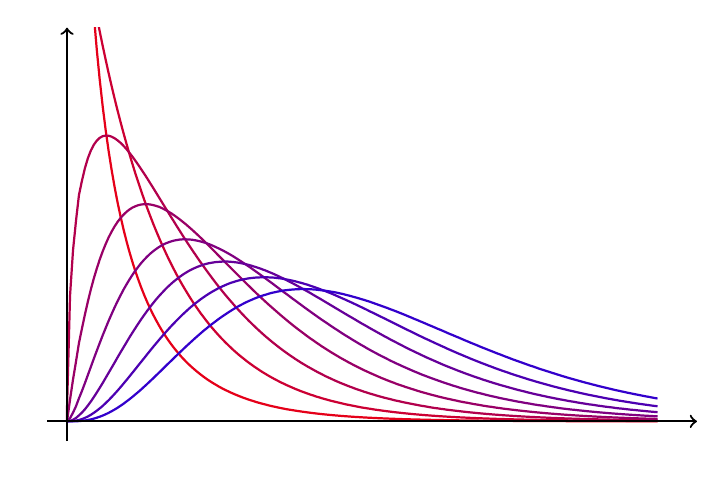
\begin{tikzpicture}[domain=.001:15,samples=200,thick,scale=0.5]
		\clip (-1,-1) rectangle (16,10);
		\foreach[count=\k,evaluate={\z=\k>2?"(0,0)--":"";\c=10*\k}] 
		\g in {sqrt(pi),1,sqrt(pi)/2,1,3/4*sqrt(pi),2,15/8*sqrt(pi),6}
		\draw[color=blue!\c!red,yscale=30] \z 
		plot (\x,{exp(ln(\x/2)*\k/2-ln(\x)-\x/2-ln(\g))});
		\draw[->] (-0.5,0) -- (16,0);
		\draw [->] (0,-0.5) -- (0,10);
	\end{tikzpicture}
	\caption{Courbe de $\chi^2(n)$ pour différentes valeurs $n$.}
\end{figure}


En remplaçant la moyenne $\mu$ par la moyenne empirique $\overline{X}$, on obtient le résultat (admis) suivant :

\begin{theoreme}{Fisher}{th_fisher}
	Si $X_1,...,X_n$ une suite de $n$ variables aléatoires indépendantes suivant chacune une même loi normale de moyenne $\mu$ et d'écart type $\sigma$. On note $$\overline{X}=\frac{1}{n}\sum_{i=1}^n X_i$$
	Alors la variable aléatoire 
	$$V =  \sum_{i=1}^{n} \left(\frac{X_i-\overline{X}}{\sigma} \right)^2$$
	suit une loi $\chi^2(n-1)$.
	De plus, la variable $\frac{\overline{X}-\mu}{\frac{\sigma}{\sqrt{n}}}$ suit une loi $\mathcal{N}(0,1)$ et est indépendante de $V$. 
\end{theoreme}

\subsection{Loi de Student}
\begin{definition}{}{}
	On considère une variable $Z \sim \mathcal{N}(0,1)$ et $U \sim \chi^2(n)$. On suppose que $Z$ et $U$ sont indépendantes. Alors la variable $$T=\frac{Z}{\sqrt{\frac{U}{n}}}$$ suit une loi de Student à $n$ degrés de liberté $St(n)$.
\end{definition}

De même que pour la loi du Chi-deux, on ne retiendra que ses paramètres pour une utilisation en statistiques.

\begin{proposition}{}{}
	Si $T$ suit une loi $St(n)$ alors 
	\begin{itemize}
		\item $\mathbb{E}(T) = 0$
		\item $\sigma^2(T)=\frac{n}{n-2}$ si $n>2$.
	\end{itemize}
\end{proposition}

\begin{figure}[h!]
	\centering
	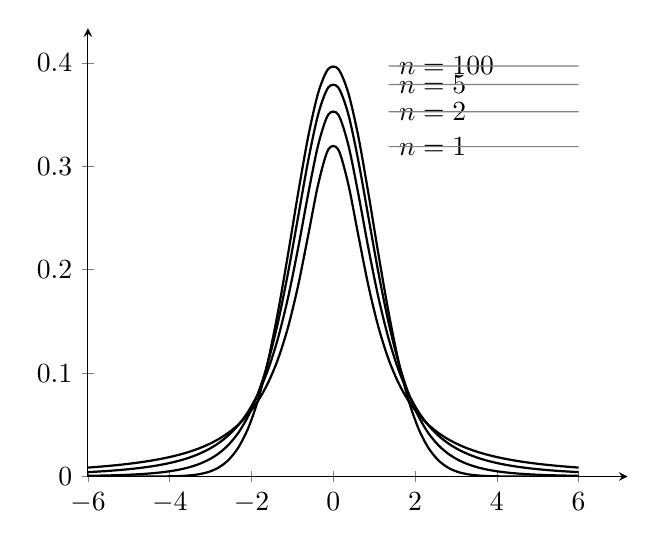
\begin{tikzpicture}[
		declare function={gamma(\z)=
			2.506628274631*sqrt(1/\z)+ 0.20888568*(1/\z)^(1.5)+ 0.00870357*(1/\z)^(2.5)- (174.2106599*(1/\z)^(3.5))/25920- (715.6423511*(1/\z)^(4.5))/1244160)*exp((-ln(1/\z)-1)*\z;},
		declare function={student(\x,\n)= gamma((\n+1)/2.)/(sqrt(\n*pi) *gamma(\n/2.)) *((1+(\x*\x)/\n)^(-(\n+1)/2.));}
		]
		
		\begin{axis}[
			axis lines=left,
			enlargelimits=upper,
			samples=50
			]
			\pgfplotsinvokeforeach{1,2,5,100}{
				\addplot [thick, smooth, domain=-6:6] {student(x,#1)} node [pos=0.5, anchor=mid west, xshift=2em, append after command={(\tikzlastnode.west) edge [thin, gray] +(-2em,0)}] {$n=#1$};
			}
		\end{axis}
	\end{tikzpicture}
	\caption{Courbe de $St(n)$ pour différentes valeurs de $n$.  }
\end{figure}

\begin{theoreme}{}{}
 Soit une suite de variables aléatoires $(T_n)$  telle que pour tout entier $n \geq 1$, $T_n$ suit une loi de Student $St(n)$. Alors $(T_n)$ converge en loi vers une loi normale $\mathcal{N}(0,1)$.
\end{theoreme}
\begin{proof}
  Soit $(Z_n)$ une suite de variables aléatoires i.i.d. selon une loi normale $\mathcal{N}(0,1)$. Ainsi, $T_n$ suit la même loi que la variable 
  $$T_n' = \frac{Z_0}{\sqrt{\frac{\sum_{k=1}^n Z_k^2}{n}}}$$
  
  Or d'après la loi forte des grands nombres, $ \frac{1}{n}\sum_{k=1}^n Z_k^2 \xrightarrow[n\to+\infty]{p.s.} \mathbb{E}(Z_0^2) = 1$.
  
  Donc la suite $(T_n')$ converge presque sûrement vers $Z_0$. D'après la propriété \ref{pr:convpsprobaloi}, la suite 
 $(T_n')$ converge en loi vers $Z_0$. Or $T_n$ a la même loi que $T_n'$, d'où la convergence en loi vers la loi de $Z_0$.
\end{proof}

Ce théorème permet de justifier que la table de valeurs fournie donne des résultats pour des lois de Student $St(n)$ avec $n \leq 30$. Au delà, on utilise une approximation par une loi normale centrée réduite. \href{https://www.geogebra.org/m/IvVDw5y3}{Voir une animation.}


\subsection{Loi de Fisher}
\begin{definition}{}{}
	On considère deux variables aléatoires indépendantes $U_1,U_2$ où  $U_1 \sim \chi^2(n_1)$ et $U_2 \sim \chi^2(n_2)$. Alors la variable $$F=\frac{U_1/n_1}{U_2/n_2}$$ suit une loi de Fisher à $n_1$ et $n_2$ degrés de liberté $F(n_1,n_2)$.
\end{definition}



\section{\'Echantillon aléatoire et estimateur ponctuel}

Le but d'une étude statistique est d'obtenir des informations sur l'ensemble d'une population. Lorsque celle-ci est de taille trop importante, on étudie un \trouer{échantillon} qui doit être prélevé de manière \trouer{aléatoire}. Ainsi, un échantillon sera modélisé par des variables aléatoires et la théorie de l'échantillonnage se basera sur la théorie des probabilités.

On considère par la suite qu'un tirage d'un échantillon de taille $n$ se fait \trouer{avec remise}, ce qui a pour conséquence que les tirages sont supposés \trouer{indépendants}.

\subsection{Définition}
\begin{definition}{}{}
	Soit $X$ une variable aléatoire définie sur un espace probabilisé $\Omega$. Un \trouer{échantillon} de taille $n$ de $X$ est un $n$-uplet $(X_1,...,X_n)$ de variables aléatoires i.i.d. suivant la même loi que $X$ (appelée loi mère). 
	
	Une \trouer{réalisation} de cet échantillon est un $n$-uplet de réels $(x_1,...,x_n)$ où pour tout $i \in [1;n]$, $X_i(\omega)=x_i$ avec $\omega \in \Omega$.
\end{definition}

\begin{definition}{}{}
	Une \trouer{statistique} d'échantillonnage est une fonction de $(X_1,...,X_n)$.
\end{definition}

\subsection{Estimateurs ponctuels}



Dans une population donnée, on considère un paramètre inconnu $\theta$ que l'on souhaite estimer (cela peut être sa moyenne, son écart-type, ou une proportion...). Soit $(X_1,...,X_n)$ un échantillon de taille $n$ de cette population.

\begin{definition}{}{}
	Un \trouer{estimateur} de $\theta$ est une statistique $T_n$ des variables $(X_1,...,X_n)$ dont la réalisation (oscillant autour de $\mathbb{E}(T)$) est envisagée comme une \og bonne \fg{} valeur de $\theta$. Si $(x_1,...,x_n)$ est une réalisation de cet échantillon, alors $T_n(x_1,...,x_n)$ est un réel appelé \trouer{estimation} du paramètre $\theta$.
\end{definition}

Il existe une infinité d'estimateurs, mais certains choix d'estimateurs ont de bonnes propriétés que l'on détaillera par la suite.

\begin{exemple}{}{}
	Un sondage effectué sur 300 votants d'une population de 50000 personnes a montré que 165 personnes sont prêtes à voter pour un candidat C. La proportion observée $p=\frac{165}{300}$ est une estimation de la proportion de votants prêts à voter pour le candidat C de la population de 50000 personnes.  Cette estimation est obtenue à l'aide de l'estimateur $F=\frac{1}{300}\sum_{i=1}^{300} X_i$.
\end{exemple}


\subsection{Propriétés attendues}


\begin{definition}{}{}
	Soit $T$ un estimateur d'un paramètre $\theta$.
	\begin{enumerate}
		\item Le \trouer{biais} de $T$ est la valeur $\mathbb{E}(T-\theta)$ notée $B(T)$ ;
		\item L'\trouer{écart quadratique moyen} est la valeur $\mathbb{E}\left((T-\theta)^2\right)$ notée $EQM(T)$
	\end{enumerate}
	
\end{definition}

Voici deux caractéristiques souhaitables pour un estimateur :

\begin{definition}{}{}
	Soit $T_n$ un estimateur d'un paramètre $\theta$ associé à un échantillon de taille $n$.
	\begin{enumerate}
		\item L'estimateur $T_n$ est \trouer{sans biais} si $B(T_n)=0$.
		\item L'estimateur $T_n$ est \trouer{asymptotiquement sans biais} si $\lim\limits_{n \to +\infty}B(T_n)=0$.
		\item L'estimateur $T_n$ \trouer{converge en moyenne quadratique} si $\lim\limits_{n \to +\infty} EQM(T_n) = 0$.
	\end{enumerate}
	
\end{definition}

\begin{proposition}{}{}
	Soit $T_n$ un estimateur d'un paramètre $\theta$ associé à un échantillon de taille $n$.
	
	$$EQM(T_n)=\sigma^2(T_n) + B(T_n)^2$$
\end{proposition}

Conséquences et interprétations :

\begin{enumerate}
	\item un estimateur converge en moyenne quadrique si et seulement s'il est asymptotiquement sans biais et sa variance tend vers $0$.
\item Plus l'écart quadratique moyen d'un estimateur est petit, meilleure est \trouer{l'efficacité} de l'estimateur.
\end{enumerate}







\subsection{Moyenne empirique}
On considère par la suite un $n$-échantillon $(X_1,...,X_n)$ de $X$.

\begin{definition}{}{}
La \trouer{moyenne empirique} de l'échantillon $(X_1,...,X_n)$ est la statistique notée $\overline{X}$ définie par 
$$\overline{X}=\frac{1}{n}\sum_{i=1}^n X_i$$
\end{definition}

\begin{proposition}{}{}
 Soit $\mu=\EX$ et $\sigma^2=V(X)$ où $X$ est la variable mère de l'échantillon $(X_1,...,X_n)$ et $\overline{X}$ la moyenne empirique de cet échantillon. Alors on a :
 \begin{itemize}
  \item $\mathbb{E}(\overline{X})=\mu$
  \item $V(\overline{X}) = \frac{\sigma^2}{n}$
 \end{itemize}
\end{proposition}
\begin{proof}
 Par linéarité de l'espérance, on a que $$\mathbb{E}(\overline{X})=\frac{1}{n}\sum_{i=1}^n \mathbb{E}(X_i)=\frac{1}{n}\sum_{i=1}^n \mathbb{E}(X) = \frac{1}{n} \times n \times \mathbb{E}(X) = \mu$$
 
 Par indépendance des variables $X_1,...,X_n$, on a  $\sigma^2(X_1+...+X_n)=\sigma^2(X_1)+...+\sigma^2(X_n) = n \sigma^2$, d'où le résultat.
\end{proof}

\subsection{Variance empirique}
\begin{definition}{}{}
La \trouer{variance empirique} de l'échantillon $(X_1,...,X_n)$ est la statistique notée $\tilde{S}^2$ définie par 
$$\tilde{S}^2=\frac{1}{n}\sum_{i=1}^n (X_i-\overline{X})^2$$
\end{definition}

\begin{proposition}{}{}
 Soit $\mu=\EX$ et $\sigma^2=V(X)$ où $X$ est la variable mère de l'échantillon $(X_1,...,X_n)$ et  $\tilde{S}^2$ la variance empirique de cet échantillon. Alors on a :
  $$\mathbb{E}(\tilde{S}^2)=\frac{n-1}{n} \sigma^2$$
\end{proposition}
\begin{proof}
 Pour faire apparaître $\sigma^2 = \frac{1}{n}\sum_{i=1}^n (X_i-\mu)^2$ dans l'expression de $\tilde{S}^2$, on écrit d'abord que pour tout $i$, $X_i-\overline{X} = X_i-\mu -(\overline{X}-\mu)$. Cela permet d'obtenir que 
 \begin{eqnarray*}
  \sum_{i=1}^n (X_i-\overline{X})^2 & = & \sum_{i=1}^n (X_i-\mu -(\overline{X}-\mu))^2 \\
                           & = & \sum_{i=1}^n (X_i-\mu)^2-2 \sum_{i=1}^n (X_i-\mu) (\overline{X}-\mu) + \sum_{i=1}^n(\overline{X}-\mu)^2\\
                           & = & \sum_{i=1}^n (X_i-\mu)^2-2 (\overline{X}-\mu)\sum_{i=1}^n (X_i-\mu)  + n(\overline{X}-\mu)^2\\
                           & = & \sum_{i=1}^n (X_i-\mu)^2-2 (\overline{X}-\mu) \times n (\overline{X}-\mu)  + n(\overline{X}-\mu)^2\\
                           & = & \sum_{i=1}^n (X_i-\mu)^2- n(\overline{X}-\mu)^2\\
 \end{eqnarray*}
Par linéarité de l'espérance, on en déduit que 
\begin{eqnarray*}
 \mathbb{E}(\tilde{S}^2) & = & \frac{1}{n} \mathbb{E}\left(\sum_{i=1}^n (X_i-\mu)^2\right)-\mathbb{E}\left((\overline{X}-\mu)^2 \right) \\
                 & = & \frac{1}{n} \sum_{i=1}^n \mathbb{E}\left( (X_i-\mu)^2\right)-\mathbb{E}\left((\overline{X}-\mu)^2 \right) \\
                 & = & \frac{1}{n} \sum_{i=1}^n \sigma^2(X_i)- \sigma^2(\overline{X}) \\
                 & = & \frac{1}{n} \sum_{i=1}^n \sigma^2-  \frac{\sigma^2}{n} \\
                % & = & \sigma^2- \frac{\sigma^2}{n}\\
                 & = & \frac{n-1}{n} \sigma^2 
\end{eqnarray*}
\end{proof}

\subsection{Fréquence}

Lorsque la variable mère suit une loi de Bernoulli (succès ou échec), on s'intéressera à la fréquence de succès dans l'échantillon à l'aide de la statistique 
$$F=\frac{1}{n}\sum_{i=1}^n X_i$$
appelée \trouer{fréquence empirique}.

\begin{proposition}{}{}
  Soit $p$ le paramètre de la loi de Bernoulli suivie par la variable mère $X$ de l'échantillon $(X_1,...,X_n)$. Soit $F$ la fréquence empirique de cet échantillon. Alors on a :
 \begin{itemize}
  \item $\mathbb{E}(F)=p$
  \item $V(F) = \frac{p(1-p)}{n}$
 \end{itemize}
\end{proposition}




Lors d'un sondage sur 1000 personnes, on peut observer la fréquence d'apparition d'un caractère $f$. On dit que $f$ est une \trouer{estimation ponctuelle} de la proportion $p$ de ce caractère dans la population mère, de taille trop importante pour être étudiée directement. On pourra également estimer la valeur de $p$ à l'aide d'une fourchette $[p_1;p_2]$ appelé intervalle de confiance.

%%%%%%%%%%%%%%%%%%%%%%%%%%%%%%%%%%%%%%%%%%%%%%%%%%%%%%%%%%%%%%%%
\subsection{Résumé sur les estimateurs usuels}
On considère un $n$-échantillon $(X_1,...,X_n)$ de moyenne $\mu$ et d'écart-type $\sigma$. Les propriétés des statistiques étudiées précédemment permettent les conclusions suivantes :

\begin{description}
 \item[Moyenne :] $\overline{X}=\frac{1}{n}\sum_{i=1}^n X_i$ est un estimateur de la moyenne $\mu$, c'est un estimateur \trouer{sans biais} et \trouer{convergent}.
 \item[Variance :] on a 3 estimateurs usuels :
 \begin{enumerate}
  \item si $\mu$ est connu, $\Sigma^2=\frac{1}{n}\sum_{i=1}^n (X_i-\mu)^2$ est un estimateur de la variance $\sigma^2$, c'est un estimateur \trouer{sans biais} et \trouer{convergent}.
  \item si $\mu$ est inconnu, $\tilde{S}^2=\frac{1}{n}\sum_{i=1}^n (X_i-\overline{X})^2$ est un estimateur de la variance $\sigma^2$, c'est un estimateur \trouer{biaisé} mais \trouer{convergent}.
  \item si $\mu$ est inconnu, $S^2=\frac{1}{n-1}\sum_{i=1}^n (X_i-\overline{X})^2 = \frac{n}{n-1}\tilde{S}^2$ est un estimateur de la variance $\sigma^2$, c'est un estimateur \trouer{sans biais} et \trouer{convergent}.
 \end{enumerate}
  \item[Fréquence :]  $F=\frac{1}{n}\sum_{i=1}^n X_i$, associé à une variable de Bernoulli de paramètre $p$, 
 est un estimateur de la fréquence de succès $p$, c'est un estimateur \trouer{sans biais} et \trouer{convergent}.
\end{description}

\section{Estimation par maximum de vraisemblance}
Les estimateurs utilisés précédemment ont été construits de manière empirique. Il existe des méthodes plus globales pour construire des estimateurs, en voici une basée sur le principe suivant : on cherche un estimateur qui rend le plus probable (vraisemblable) l'échantillon observé.

%\begin{figure}[h!]
%	\centering
%	\includegraphics[width=0.5\linewidth]{maxvrais}
%	\caption[]{un exemple d'application de la théorie}
%	\label{fig:exemples}
%\end{figure}

\subsection{Fonction de vraisemblance pour une loi discrète}

On considère un échantillon $X_1,...,X_n$ de variables aléatoires indépendantes suivant une loi discrète $\mathcal{L}(\theta)$ où $\theta$ est le paramètre que l'on cherche à estimer. On note $x_1,...,x_n$ une réalisation de l'échantillon. On s'intéresse à l'événement : 
$$A = \{X_1=x_1,...,X_n=x_n\}$$

La \trouer{fonction de vraisemblance} $L(x_1,...,x_n, \theta)$ est la probabilité de cet événement, autrement dit la probabilité que l'échantillon se réalise tel qu'on l'a observé. Par indépendance des variables aléatoires, on obtient :

$$L(x_1,...,x_n, \theta) = \prob_\theta(A) = \prob_\theta(X_1=x_1) \times ... \times \prob_\theta(X_n=x_n)$$

On notera que le calcul de probabilité dépend du paramètre $\theta$ que l'on cherche à estimer, puisque la loi $\mathcal{L}(\theta)$ dépend de ce paramètre.

\subsection{Fonction de vraisemblance pour une loi continue}

On considère un échantillon $X_1,...,X_n$ de variables aléatoires indépendantes suivant une loi continue $\mathcal{L}(\theta)$ où $\theta$ est le paramètre que l'on cherche à estimer. On note $x_1,...,x_n$ une réalisation de l'échantillon. L'événement $\{X_i=x_i\}$ étant de probabilité nulle pour une loi continue, on s'intéresse plutôt à l'événement $\{|X_i-x_i|<\varepsilon\}$. Supposons que la loi $\mathcal{L}(\theta)$ admette une densité $f_{\theta}$ : alors $\prob_{\theta}(|X_i-x_i|<\varepsilon) = \int_{x_i-\varepsilon}^{x_i+\varepsilon} f_{\theta}$. D'après le théorème de la moyenne, il existe $c \in ]x_i-\varepsilon;x_i+\varepsilon[$ tel que $f_{\theta}(c) = \frac{1}{2\varepsilon} \prob_{\theta}(|X_i-x_i|<\varepsilon)$. Par continuité, on peut écrire $f_{\theta}(c) = f_{\theta}(x_i)+\alpha_i(\varepsilon)$ où $\alpha_i(\varepsilon)$ tend vers $0$ lorsque $\varepsilon \to 0$. 

De manière analogue au cas discret, on s'intéresse donc à l'événement 
$$A_{\varepsilon} = \{|X_1-x_1|<\varepsilon,...,|X_n-x_n|<\varepsilon\}$$

Or $$ \frac{1}{2\varepsilon} \prob_{\theta}\left(A_{\varepsilon}\right) = \left(f_{\theta}(x_1)+\alpha_1(\varepsilon)\right) \times ... \times \left(f_{\theta}(x_n)+\alpha_n(\varepsilon)\right)$$

En faisant tendre $\varepsilon \to 0$, on définit donc la fonction de vraisemblance 

$$L(x_1,...,x_n, \theta) = \prob_\theta(A_{\varepsilon}) = f_{\theta}(x_1) \times ... \times f_{\theta}(x_n)$$

\subsection{Optimiser la vraisemblance}

On cherche une valeur de $\theta$ telle que la vraisemblance soit maximale. Lorsque cela est possible, on cherche $\theta$ tel que 

$${\frac {\partial L(x_{1},\ldots ,x_{i},\ldots ,x_{n};\theta )}{\partial \theta }}=0 $$
De manière équivalente, on cherche le maximum de la \trouer{log-vraisemblance} :
$${\frac {\partial \ln L(x_{1},\ldots ,x_{i},\ldots ,x_{n};\theta )}{\partial \theta }}=0 $$

ce qui peut conduire à des calculs plus simples. 

\begin{definition}{}{}
	L'estimation du maximum de vraisemblance est, lorsqu'elle existe, la valeur $\hat{\theta}$ qui maximise la fonction $\theta \mapsto L(x_1,...,x_n, \theta)$. 
\end{definition}

L'estimation $\hat{\theta}$ dépend des réalisations $x_1,...,x_n$. Pour obtenir l'estimateur $\Theta$ recherché, on remplace dans l'expression les réalisations $x_1,...,x_n$ par les variables aléatoires $X_1,...,X_n$.

\subsection{Exemple : estimer le paramètre d'une loi de Bernoulli}

On considère un échantillon $X_1,...,X_n$ de variables aléatoires indépendantes suivant une loi de Bernoulli de paramètre $p$ inconnu. Soit $x_1,...,x_n$ une réalisation de cet échantillon :

$$\prob_p(X_i=x_i)=\left\{\begin{array}{cl}
p&\text{si $x_i = 1$}\\
1-p &\text{si $x_i = 0$}
\end{array}\right.$$

Par indépendance, la fonction de vraisemblance devient alors :

$$L(x_1,...,x_n, p) = p^{\sum_{i=1}^n x_i} \times \left(1-p\right)^{n-\sum_{i=1}^n x_i}$$

Cette fonction de $p$ est strictement positive sur $]0;1[$, nulle pour $p \in \{0;1\}$. Elle admet un maximum pour une valeur $\hat{p} \in ]0;1[$. En supposant que $p \notin \{0;1\}$, il est plus commode de considérer le logarithme de cette expression :

$$\ln L(x_1,...,x_n, p) = \left(\sum_{i=1}^n x_i \right) \ln(p) + \left(n-\sum_{i=1}^n x_i \right) \ln(1-p)$$

puis de chercher à annuler sa dérivée :

$$\frac {\partial \ln L(x_{1},\ldots ,x_{i},\ldots ,x_{n};p )}{\partial p } = \frac{\sum_{i=1}^n x_i}{p} - \frac{n - \sum_{i=1}^n x_i}{1-p} = 0 \iff p = \frac{1}{n } \sum_{i=1}^n x_i$$

On trouve donc une valeur $\hat{p} = \frac{1}{n } \sum_{i=1}^n x_i$. On en déduit un estimateur de $p$ qui est l'estimateur de fréquence déjà connu :

$$F = \frac{1}{n } \sum_{i=1}^n X_i$$


\section{Estimation par intervalle de confiance}
On cherche maintenant à estimer un paramètre à l'aide d'un intervalle. Cela  permet de contrôler l'erreur lors de l'estimation.

\subsection{Démarche générale}
\'Etant donné un estimateur $T$ d'un paramètre $\theta$ et un niveau de confiance $(1-\alpha)$ où $\alpha \in ]0;1[$, on cherche à déterminer un intervalle $I_{conf}(T)$ tel que 
$$\prob\left(\theta \in I_{conf}(T)\right) = 1-\alpha$$

Le nombre $\alpha$ est le \trouer{risque d'erreur}, on choisit souvent $\alpha = 5\%$ ou $\alpha = 1\%$.

On cherche autant que possible à déterminer des intervalles de confiance à \trouer{risques symétriques}, c'est-à-dire des intervalles de la forme $[T-\epsilon;T+\epsilon]$ avec 
$$\prob(\theta < T-\epsilon) = \prob(\theta > T+\epsilon) = \frac{\alpha}{2}$$

Pour calculer ces probabilités, il faut connaître en particulier les lois suivies par les estimateurs usuels (on rappelle qu'un estimateur est avant tout une variable aléatoire).

\subsection{Intervalle de confiance asymptotique}
Un intervalle de confiance asymptotique au niveau $1-\alpha$ est un intervalle $I_{n}(T)$ tel que 
$$\lim_{n \to +\infty} \prob\left(\theta \in I_{n}(T)\right) = 1-\alpha$$

En pratique, on utilise un tel intervalle << quand $n$ est grand >>. Cette situation se produit notamment lorsque l'on approche la loi de l'estimateur à l'aide du théorème central limite.

\subsection{Intervalle de confiance asymptotique d'une proportion}
\paragraph{Estimateur utilisé :} Soit $F=\frac{1}{n}\sum_{i=1}^n X_i$ l'estimateur de fréquence associé à une variable de Bernoulli de paramètre $p$. Alors la variable $nF$ suit une loi binomiale $\mathscr{B}(n,p)$ et on en déduit que  $\mathbb{E}(F)=p$
et $\sigma^2(F) = \frac{p(1-p)}{n}$.

\paragraph{Loi de l'estimateur utilisée :}  On suppose que $n>30$, $np>5$ et $n(1-p)>5$. D'après le théorème central limite, on sait donc que $F$ peut-être approché par une loi normale $\mathcal{N}\left(p,\frac{p(1-p)}{n}\right)$. 

\paragraph{Calcul d'un intervalle de confiance asymptotique :}  On sait que $\frac{F-p}{\sqrt{\frac{p(1-p)}{n}}}$ suit approximativement une loi normale centrée réduite $\mathcal{N}(0,1)$. On rappelle qu'il existe un unique réel strictement positif $u_{\alpha/2}$ tel que 

$$\prob(-u_{\alpha/2} < Z < u_{\alpha/2}) = 1-\alpha$$
où $Z=\frac{F-p}{\sqrt{\frac{p(1-p)}{n}}}$ suit une loi $\mathcal{N}(0,1)$.

Or \begin{eqnarray*}
	-u_{\alpha/2} \leq Z \leq u_{\alpha/2} & \iff & -u_{\alpha/2} \leq \frac{F-p}{\sqrt{\frac{p(1-p)}{n}}} \leq u_{\alpha/2} \\
	& \iff & F-u_{\alpha/2} {\sqrt{\frac{p(1-p)}{n}}}  \leq p \leq F + u_{\alpha/2}{\sqrt{\frac{p(1-p)}{n}}} \\
	& \iff & p \in I_{conf}(F)
\end{eqnarray*}
où $$I_{conf}(F)=\left[F-u_{\alpha/2} {\sqrt{\frac{p(1-p)}{n}}} ~;~ F + u_{\alpha/2}{\sqrt{\frac{p(1-p)}{n}}} \right]$$ 

Cet intervalle aléatoire contient la valeur $p$ recherchée avec une probabilité $1-\alpha$. 

Un intervalle de confiance est aussi une \textit{réalisation} de cet intervalle aléatoire à partir des données observées. La réalisation $F(\omega)$ de la variable $F$ est dite << fréquence observée dans l'échantillon >> que l'on note également $f_{obs}$. La réalisation de cet intervalle est donc :
$$\left[f_{obs}-u_{\alpha/2} {\sqrt{\frac{p(1-p)}{n}}} ~;~ f_{obs} + u_{\alpha/2}{\sqrt{\frac{p(1-p)}{n}}} \right]$$

\paragraph{Modification de l'intervalle avec des données connues :}

Le problème de l'intervalle de confiance trouvé ici est que ses bornes dépendent du paramètre \trouer{inconnu} $p$. L'écart-type $\tilde{\sigma}=\sqrt{\frac{f(1-f)}{n}}$ associé à la fréquence observée est un estimateur de l'écart-type $\sigma=\sqrt{\frac{p(1-p)}{n}}$ mais il est biaisé, on peut en revanche estimer $\sigma$ par $\sqrt{\frac{n}{n-1}}\tilde{\sigma}$. On peut donc prendre pour intervalle de confiance :

$$I_{conf}(F(\omega))=\left[f_{obs}-u_{\alpha/2} \sqrt{\frac{f_{obs}(1-f_{obs})}{n-1}} ~;~ f_{obs} + u_{\alpha/2} \sqrt{\frac{f_{obs}(1-f_{obs})}{n-1}} \right]$$

\paragraph{En pratique :} 
\begin{enumerate}
	\item Dans une situation courante : si $n$ est grand, on peut remplacer $n-1$ par $n$ :
	
	$$I_{conf}(F(\omega))=\left[f_{obs}-u_{\alpha/2} \sqrt{\frac{f_{obs}(1-f_{obs})}{n}} ~;~ f_{obs} + u_{\alpha/2} \sqrt{\frac{f_{obs}(1-f_{obs})}{n}} \right]$$
	Cet intervalle, dit << intervalle de Wald >>, comporte des défauts statistiques mais est très communément utilisé.
	\item  Si $f_{obs}$ n'est pas connu et qu'on s'intéresse seulement à la longueur de l'intervalle, on peut majorer $p(1-p)$ par $0{,}25$, on obtient ainsi un intervalle de confiance par excès de $p$ :
	
	$$I_{conf}(F(\omega))=\left[ f_{obs}-u_{\alpha/2} \frac{1}{2 \sqrt{n}} ~;~ f_{obs} + u_{\alpha/2} \frac{1}{2 \sqrt{n}} \right]$$
	Ce résultat est d'autant plus pertinent que $p(1-p)$ est proche de son maximum, c'est-à-dire si $p$ est proche de $0.5$.
	
	Dans ce cas, la longueur de l'intervalle est $u_{\alpha/2} \frac{1}{\sqrt{n}}$. Cette quantité ne dépend que de la taille de l'échantillon et du niveau de confiance souhaité. 
	
\end{enumerate}



\subsection{Intervalle de confiance d'une moyenne}
\paragraph{Estimateur utilisé :} Soit $\overline{X}=\frac{1}{n}\sum_{i=1}^n X_i$ l'estimateur de la moyenne $\mu$ pour une loi mère de moyenne $\mu$ et d'écart-type $\sigma$. On a calculé que $\mathbb{E}(\overline{X})=\mu$
et $\sigma^2(\overline{X}) = \frac{\sigma^2}{n}$.

\paragraph{Loi de l'estimateur utilisé :}  

\begin{enumerate}
	\item Si l'échantillon est distribué normalement selon une $\mathcal{N}\left(\mu,\sigma^2\right)$ alors $\overline{X}$ suit (exactement) une loi $\mathcal{N}\left(\mu,\frac{\sigma^2}{n}\right)$.
	\item Si on ne sait pas que l'échantillon est distribué normalement et que $n$ est considéré comme grand, on peut considérer que $\overline{X}$ suit approximativement une loi normale $\mathcal{N}\left(\mu,\frac{\sigma^2}{n}\right)$ d'après le théorème central limite.
\end{enumerate}


\paragraph{Calcul d'un intervalle de confiance pour cette loi :}  On sait que $\frac{\overline{X}-\mu}{\frac{\sigma}{\sqrt{n}}}$ suit une loi normale centrée réduite $\mathcal{N}(0,1)$. De même que précédemment, il existe un unique réel strictement positif $u_{\alpha/2}$ tel que 

$$\prob\left(\overline{X}-u_{\alpha/2} \frac{\sigma}{\sqrt{n}} < \mu < \overline{X} + u_{\alpha/2} \frac{\sigma}{\sqrt{n}}\right) = 1-\alpha$$

d'où $$I_{conf}(\overline{X})=\left[\overline{X}-u_{\alpha/2} \frac{\sigma}{\sqrt{n}}~;~\overline{X} + u_{\alpha/2} \frac{\sigma}{\sqrt{n}} \right]$$
On note $x_{obs}=\overline{X}(\omega)$ la moyenne observée dans l'échantillon, c'est une réalisation de la variable $\overline{X}$.

\subsection{Intervalle de confiance d'une moyenne, l'écart-type est inconnu}
Le calcul précédent est possible en connaissant l'écart-type $\sigma$ de la loi mère. En général, quand on cherche la moyenne $\mu$, l'écart-type $\sigma$ est également inconnu. 

\paragraph{Estimateur utilisé :} On fait intervenir un estimateur de $\sigma^2$, ici l'estimateur usuel non biaisé $$S^2=\frac{1}{n-1}\sum_{i=1}^n (X_i-\overline{X})^2$$

\paragraph{Loi de l'estimateur utilisé si la loi mère a une distribution normale :} on sait donc que $Z=\frac{\overline{X}-\mu}{\frac{\sigma}{\sqrt{n}}}$ suit une loi normale $\mathcal{N}\left(0,1 \right)$. En remplaçant $\sigma$ par l'estimateur $S$, 
d'après la définition d'une loi de Student et le théorème de Fisher (th \ref{th:th_fisher})
 $$\frac{Z}{\sqrt{\frac{\frac{(n-1)}{\sigma^2}S^2}{n-1}}}$$ suit une loi $St(n-1)$.  En remplaçant $Z$ par son expression et en simplifiant, il vient que $U=\frac{\overline{X}-\mu}{\frac{S}{\sqrt{n}}}$ suit une loi $St(n-1)$.

\paragraph{Calcul d'un intervalle de confiance pour cette loi :} De même que pour une loi normale, il existe un unique réel strictement positif $t_{\alpha/2}$ tel que 

$$\prob(-t_{\alpha/2} < U < t_{\alpha/2}) = 1-\alpha$$

On en déduit un intervalle de confiance asymptotique :

$$I_{conf}(\overline{X})=\left[\overline{X}-t_{\alpha/2} \frac{S}{\sqrt{n}}~;~\overline{X} + t_{\alpha/2} \frac{S}{\sqrt{n}} \right]$$

que l'on réalise en utilisant les valeurs observées.  

\paragraph{Loi de l'estimateur utilisée si la loi mère a une distribution quelconque et $n$ est grand :} d'après le théorème central limite, la variable  $Z=\frac{\overline{X}-\mu}{\frac{\sigma}{\sqrt{n}}}$ suit approximativement une loi normale $\mathcal{N}\left(0,1 \right)$. On admet qu'alors, en remplaçant $\sigma$ par son estimateur $S$, $U=\frac{\overline{X}-\mu}{\frac{S}{\sqrt{n}}}$ suit approximativement une loi $\mathcal{N}\left(0,1 \right)$.

On en déduit un intervalle de confiance :

$$I_{conf}(\overline{X})=\left[\overline{X}-u_{\alpha/2} \frac{S}{\sqrt{n}}~;~\overline{X} + u_{\alpha/2} \frac{S}{\sqrt{n}} \right]$$

\paragraph{Si la loi mère a une distribution quelconque et que l'échantillon n'est pas de grande taille $n$ :} on ne peut rien dire.



 \subsection{Intervalle de confiance d'une variance}
\paragraph{Estimateur utilisé :} On fait intervenir un estimateur de $\sigma^2$, en l'occurrence $$S^2=\frac{1}{n-1}\sum_{i=1}^n (X_i-\overline{X})^2$$

\paragraph{Loi de l'estimateur utilisé si la loi mère a une distribution normale :}  on a vu précédemment que la variable $\frac{(n-1)}{\sigma^2}S^2$ suit une loi $\chi^2(n-1)$, on obtient un intervalle de confiance pour estimer une variance. 

Remarquons que si la moyenne $\mu$ est connue, l'estimateur est 
$$\Sigma^2=\frac{1}{n}\sum_{i=1}^n (X_i-\mu)^2$$
et on sait que $\frac{n}{\sigma^2}\Sigma^2$ suit une loi $\chi^2(n)$.


